\documentclass[12pt,fleqn]{article}\usepackage{../../common}
\begin{document}
Green'in Teorisi, Uzaklaşım, Stokes, Yol ve Çizgi Entegralleri

Yüzeyler (Surfaces)

Üç boyut içindeki iki boyut yüzeyler parametrize edilerek gösterilir,
tek boyutlu eğri bir parametre $t$ ile parametrize ediliyordu, alan için
iki değişken $u,v$ gerekir. Notasyonel olarak $r$'nin taradığı bir yüzey

$$
r(u,v) = < x(u,v), y(u,v), z(u,v) >
$$

Mesela $r(u,v) = < u, u^2, v >$ bir yüzey olabilir.

Yüzey alan hesabı için tüm yüzeyi kenarları $\Delta u$, $\Delta v$ olan hücreler
yaratabiliriz. Her noktada iki tane teğet vektör bulunabilir, bunlar $t_u$ ve
$t_v$ olsun,

$$
t_u = < \frac{\partial x}{\partial u},
        \frac{\partial y}{\partial u},
        \frac{\partial z}{\partial u} >, \quad
t_v = < \frac{\partial x}{\partial v},
        \frac{\partial y}{\partial v},
        \frac{\partial z}{\partial v} >        
$$

Yaklaşık olarak her hücrenin alanı $\Delta S_{ij}$ her hücredeki $t_u$ ve $t_v$
(ya da yeni notasyonla onlara $t_u^{ij}$ ve $t_v^{ij}$ diyelim) yönündeki
$\Delta u$ ve $\Delta v$'nin oluşturduğu paralelogram alanıdır, bu paralelogram
bildiğimiz gibi iki vektörün çapraz çarpımından gelen üçüncü vektörün
büyüklüğüdür, o zaman 

$$
\Delta S_{ij} \approx || \Delta u t_u^{ij} \times \Delta v t_v^{ij} ||
$$

$$
= ||  t_u^{ij} \times t_v^{ij} || \Delta u \Delta v
$$
        
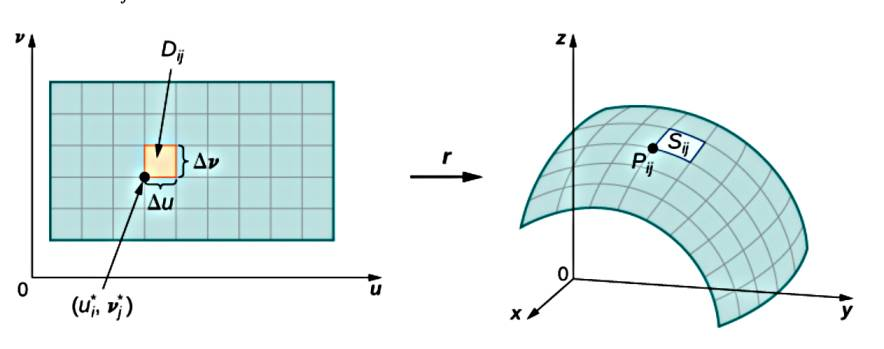
\includegraphics[width=20em]{calc_multi_75_app_01.jpg}

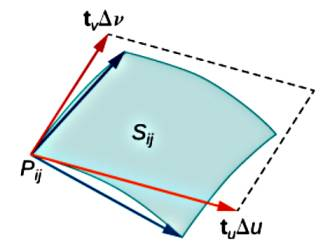
\includegraphics[width=10em]{calc_multi_75_app_02.jpg}

Tüm ufak hücre alanlarını toplarız, ve hücre sayısı sonsuza yaklaşırken toplam
alan limitine bakabiliriz,

$$
\lim_{m,n \to \infty} \sum_{i=1}^{m} \sum_{j=1}^{n} || t_u^{ij} \times t_v^{ij} || \Delta u \Delta v
$$

Bu limit yüzey alan çift entegral hesabına yaklaşır / onu tanımlar, [2, sf. 769],

$$
= \iint_D || t_u \times t_v || \ud u \ud v = \iint_D || t_u \times t_v || \ud A
$$

Yüzey Entegrali (Surface Integral)

Yukarıda gördüklerimiz parametrize edilmiş yüzeyin alanını hesaplamak içindir.
Yüzey entegrali bir yüzey {\em üzerinden} alınan entegrallere verilen isimdir,
mesela tek sayı / skalar değerli bir fonksiyon $f$'nin pürüzsüz bir yüzey $S$
üzerinden alınan yüzey entegrali, o fonksiyonun her noktadaki alan büyüklüğü ile
çarpılıp sonuçların toplanmasıdır, cebirsel olarak yine $t_u,t_v$ kavramlarını
kullanırsak,

$$
\iint_S f(x,y,z) \ud S 
= \lim_{m,n \to \infty} \sum_{i=1}^{m} \sum_{j=1}^{n} f(P_{ij}) || t_u^{ij} \times t_v^{ij} || \Delta u \Delta v
$$

$$
= \lim_{m,n \to \infty} \sum_{i=1}^{m} \sum_{j=1}^{n} f(P_{ij}) \Delta S_{ij} 
$$

O zaman yuzey entegralleri alttaki sekilde hesaplanabilir,

$$
\iint_S f(x,y,z) \ud S =
\iint_D f(r(u,v)) || t_u \times t_v || \ud A
$$

Çizgi entegrali (line integrals) daha düşük boyuttaki benzer bir kavram idi.

Vektör Alanı İçinde Yüzey Entegrali

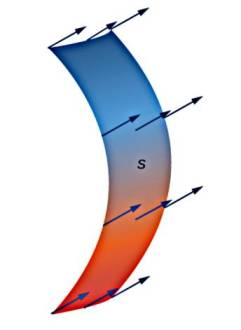
\includegraphics[width=10em]{calc_multi_75_app_04.jpg}


\begin{minted}[fontsize=\footnotesize]{python}
from mpl_toolkits.mplot3d import Axes3D
from matplotlib import cm
import numpy as np
fig = plt.figure()
ax = fig.add_subplot(111, projection='3d')
u = np.linspace(0, 3, 100)
v = np.linspace(0, 4, 100)
u,v = np.meshgrid(u,v)

x = u; y = v**2 - u; z = u + v

ax.plot_surface(x, y, z, rstride=4, cstride=4, cmap = cm.copper)
x = np.linspace(0, 3, 5)
y = np.linspace(0, 10, 5)
z = np.linspace(0, 6, 5)

fu = -y; fv = x; fw = z*0

xx,yy,zz = np.meshgrid(x,y,z)
ax.quiver(xx, yy, zz, fu, fv, fw, length=0.2, color = 'red')
ax.view_init(elev=18, azim=-46)
plt.savefig('calc_multi_75_app_03.jpg',quality=30)
\end{minted}

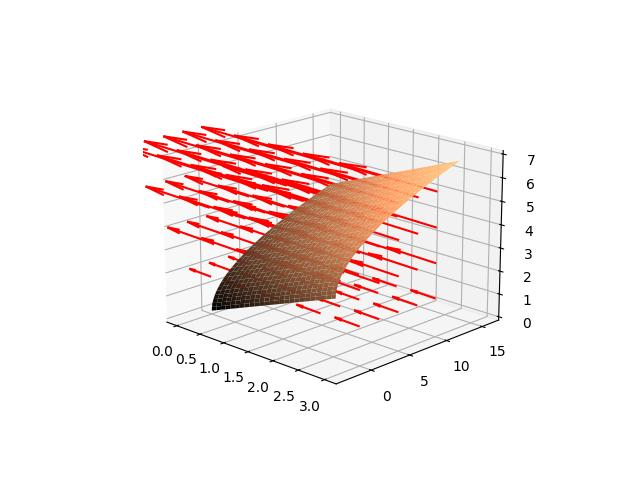
\includegraphics[width=15em]{calc_multi_75_app_03.jpg}





[devam edecek]

Kaynaklar

[1] Marsden, {\em Vector Calculus}

[2] Strang, {\em Calculus Volume 3, OpenStaxa}

\end{document}



